% Options for packages loaded elsewhere
\PassOptionsToPackage{unicode}{hyperref}
\PassOptionsToPackage{hyphens}{url}
%
\documentclass[
]{article}
\usepackage{lmodern}
\usepackage{amssymb,amsmath}
\usepackage{ifxetex,ifluatex}
\ifnum 0\ifxetex 1\fi\ifluatex 1\fi=0 % if pdftex
  \usepackage[T1]{fontenc}
  \usepackage[utf8]{inputenc}
  \usepackage{textcomp} % provide euro and other symbols
\else % if luatex or xetex
  \usepackage{unicode-math}
  \defaultfontfeatures{Scale=MatchLowercase}
  \defaultfontfeatures[\rmfamily]{Ligatures=TeX,Scale=1}
\fi
% Use upquote if available, for straight quotes in verbatim environments
\IfFileExists{upquote.sty}{\usepackage{upquote}}{}
\IfFileExists{microtype.sty}{% use microtype if available
  \usepackage[]{microtype}
  \UseMicrotypeSet[protrusion]{basicmath} % disable protrusion for tt fonts
}{}
\makeatletter
\@ifundefined{KOMAClassName}{% if non-KOMA class
  \IfFileExists{parskip.sty}{%
    \usepackage{parskip}
  }{% else
    \setlength{\parindent}{0pt}
    \setlength{\parskip}{6pt plus 2pt minus 1pt}}
}{% if KOMA class
  \KOMAoptions{parskip=half}}
\makeatother
\usepackage{xcolor}
\IfFileExists{xurl.sty}{\usepackage{xurl}}{} % add URL line breaks if available
\IfFileExists{bookmark.sty}{\usepackage{bookmark}}{\usepackage{hyperref}}
\hypersetup{
  pdftitle={Econometrics II - Problem 5},
  pdfauthor={William Radaic Peron},
  hidelinks,
  pdfcreator={LaTeX via pandoc}}
\urlstyle{same} % disable monospaced font for URLs
\usepackage[margin=1in]{geometry}
\usepackage{color}
\usepackage{fancyvrb}
\newcommand{\VerbBar}{|}
\newcommand{\VERB}{\Verb[commandchars=\\\{\}]}
\DefineVerbatimEnvironment{Highlighting}{Verbatim}{commandchars=\\\{\}}
% Add ',fontsize=\small' for more characters per line
\usepackage{framed}
\definecolor{shadecolor}{RGB}{248,248,248}
\newenvironment{Shaded}{\begin{snugshade}}{\end{snugshade}}
\newcommand{\AlertTok}[1]{\textcolor[rgb]{0.94,0.16,0.16}{#1}}
\newcommand{\AnnotationTok}[1]{\textcolor[rgb]{0.56,0.35,0.01}{\textbf{\textit{#1}}}}
\newcommand{\AttributeTok}[1]{\textcolor[rgb]{0.77,0.63,0.00}{#1}}
\newcommand{\BaseNTok}[1]{\textcolor[rgb]{0.00,0.00,0.81}{#1}}
\newcommand{\BuiltInTok}[1]{#1}
\newcommand{\CharTok}[1]{\textcolor[rgb]{0.31,0.60,0.02}{#1}}
\newcommand{\CommentTok}[1]{\textcolor[rgb]{0.56,0.35,0.01}{\textit{#1}}}
\newcommand{\CommentVarTok}[1]{\textcolor[rgb]{0.56,0.35,0.01}{\textbf{\textit{#1}}}}
\newcommand{\ConstantTok}[1]{\textcolor[rgb]{0.00,0.00,0.00}{#1}}
\newcommand{\ControlFlowTok}[1]{\textcolor[rgb]{0.13,0.29,0.53}{\textbf{#1}}}
\newcommand{\DataTypeTok}[1]{\textcolor[rgb]{0.13,0.29,0.53}{#1}}
\newcommand{\DecValTok}[1]{\textcolor[rgb]{0.00,0.00,0.81}{#1}}
\newcommand{\DocumentationTok}[1]{\textcolor[rgb]{0.56,0.35,0.01}{\textbf{\textit{#1}}}}
\newcommand{\ErrorTok}[1]{\textcolor[rgb]{0.64,0.00,0.00}{\textbf{#1}}}
\newcommand{\ExtensionTok}[1]{#1}
\newcommand{\FloatTok}[1]{\textcolor[rgb]{0.00,0.00,0.81}{#1}}
\newcommand{\FunctionTok}[1]{\textcolor[rgb]{0.00,0.00,0.00}{#1}}
\newcommand{\ImportTok}[1]{#1}
\newcommand{\InformationTok}[1]{\textcolor[rgb]{0.56,0.35,0.01}{\textbf{\textit{#1}}}}
\newcommand{\KeywordTok}[1]{\textcolor[rgb]{0.13,0.29,0.53}{\textbf{#1}}}
\newcommand{\NormalTok}[1]{#1}
\newcommand{\OperatorTok}[1]{\textcolor[rgb]{0.81,0.36,0.00}{\textbf{#1}}}
\newcommand{\OtherTok}[1]{\textcolor[rgb]{0.56,0.35,0.01}{#1}}
\newcommand{\PreprocessorTok}[1]{\textcolor[rgb]{0.56,0.35,0.01}{\textit{#1}}}
\newcommand{\RegionMarkerTok}[1]{#1}
\newcommand{\SpecialCharTok}[1]{\textcolor[rgb]{0.00,0.00,0.00}{#1}}
\newcommand{\SpecialStringTok}[1]{\textcolor[rgb]{0.31,0.60,0.02}{#1}}
\newcommand{\StringTok}[1]{\textcolor[rgb]{0.31,0.60,0.02}{#1}}
\newcommand{\VariableTok}[1]{\textcolor[rgb]{0.00,0.00,0.00}{#1}}
\newcommand{\VerbatimStringTok}[1]{\textcolor[rgb]{0.31,0.60,0.02}{#1}}
\newcommand{\WarningTok}[1]{\textcolor[rgb]{0.56,0.35,0.01}{\textbf{\textit{#1}}}}
\usepackage{graphicx,grffile}
\makeatletter
\def\maxwidth{\ifdim\Gin@nat@width>\linewidth\linewidth\else\Gin@nat@width\fi}
\def\maxheight{\ifdim\Gin@nat@height>\textheight\textheight\else\Gin@nat@height\fi}
\makeatother
% Scale images if necessary, so that they will not overflow the page
% margins by default, and it is still possible to overwrite the defaults
% using explicit options in \includegraphics[width, height, ...]{}
\setkeys{Gin}{width=\maxwidth,height=\maxheight,keepaspectratio}
% Set default figure placement to htbp
\makeatletter
\def\fps@figure{htbp}
\makeatother
\setlength{\emergencystretch}{3em} % prevent overfull lines
\providecommand{\tightlist}{%
  \setlength{\itemsep}{0pt}\setlength{\parskip}{0pt}}
\setcounter{secnumdepth}{-\maxdimen} % remove section numbering

\title{Econometrics II - Problem 5}
\author{William Radaic Peron}
\date{\today}

\begin{document}
\maketitle

In this problem, we'll be forecasting GDP in the short term and creating
some models of GDP growth in the long run. This presents some
challenges, namely those related to \emph{ergodicity} and
\emph{stationarity}.

\begin{Shaded}
\begin{Highlighting}[]
\NormalTok{pplot <-}\StringTok{ }\KeywordTok{ggplot}\NormalTok{(}\DataTypeTok{data =}\NormalTok{ pib, }\KeywordTok{aes}\NormalTok{(}\DataTypeTok{x =}\NormalTok{ t, }\DataTypeTok{y =}\NormalTok{ v)) }\OperatorTok{+}\StringTok{ }\KeywordTok{geom_line}\NormalTok{() }\OperatorTok{+}\StringTok{ }
\StringTok{    }\KeywordTok{ggtitle}\NormalTok{(}\StringTok{"Time series plot"}\NormalTok{) }\OperatorTok{+}\StringTok{ }\KeywordTok{theme_few}\NormalTok{()}
\NormalTok{pplot}
\end{Highlighting}
\end{Shaded}

\begin{center}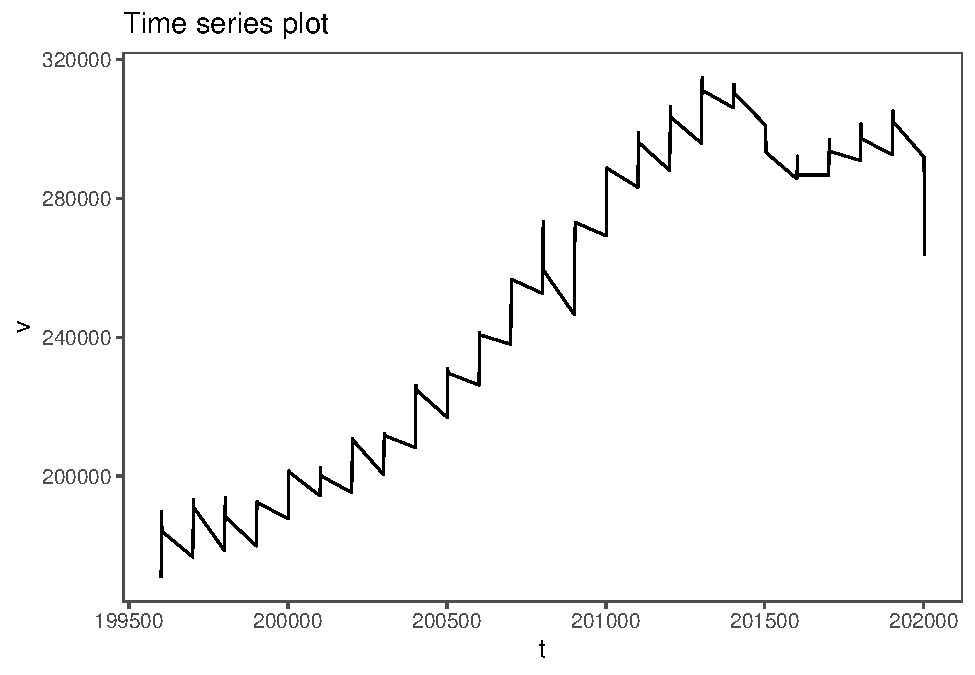
\includegraphics{Econo2_P5_files/figure-latex/plots-1} \end{center}

As we have downloaded the \emph{pure} quarterly data, it presents
\emph{seasonality} and an upwards tendency. This implies that the
\emph{time series will not be stationary}. Therefore, we need to employ
methods that circumvent this issue and assure us that we can continue
modelling the series as an ARMA(p,q).

\section{Decomposing the time series}

We will now assume that we can decompose the time series in three
distinct elements in an additive model: \[ X_t = f_t+ s_t + Y_t \],
where \(f_t\) denotes the tendency of the ts, \(s_t\) denotes
seasonality, \(Y_t\) is stochastic. We also assume that \(f_t, s_t\) are
\emph{deterministic}.

\subsection{Trend}

First, we'll construct a \emph{parametric} model of the trend. Let's
assume that \(f_t\) can be modelled by a linear form:
\[ f_t = \gamma_0 + \gamma *t \]

\begin{Shaded}
\begin{Highlighting}[]
\NormalTok{linear_trend <-}\StringTok{ }\KeywordTok{lm}\NormalTok{(v }\OperatorTok{~}\StringTok{ }\NormalTok{t, }\DataTypeTok{data =}\NormalTok{ pib)}

\KeywordTok{summary}\NormalTok{(linear_trend)}
\end{Highlighting}
\end{Shaded}

\begin{verbatim}
## 
## Call:
## lm(formula = v ~ t, data = pib)
## 
## Residuals:
##    Min     1Q Median     3Q    Max 
## -59917 -10577  -2046  11571  33717 
## 
## Coefficients:
##               Estimate Std. Error t value Pr(>|t|)    
## (Intercept) -1.194e+07  4.644e+05  -25.71   <2e-16 ***
## t            6.070e+01  2.313e+00   26.25   <2e-16 ***
## ---
## Signif. codes:  0 '***' 0.001 '**' 0.01 '*' 0.05 '.' 0.1 ' ' 1
## 
## Residual standard error: 16200 on 96 degrees of freedom
## Multiple R-squared:  0.8777, Adjusted R-squared:  0.8764 
## F-statistic: 688.8 on 1 and 96 DF,  p-value: < 2.2e-16
\end{verbatim}

\begin{Shaded}
\begin{Highlighting}[]
\KeywordTok{ggplot}\NormalTok{(}\DataTypeTok{data =}\NormalTok{ pib, }\KeywordTok{aes}\NormalTok{(}\DataTypeTok{x =}\NormalTok{ t, }\DataTypeTok{y =}\NormalTok{ v)) }\OperatorTok{+}\StringTok{ }\KeywordTok{stat_smooth}\NormalTok{(}\DataTypeTok{method =} \StringTok{"lm"}\NormalTok{, }
    \DataTypeTok{se =}\NormalTok{ F) }\OperatorTok{+}\StringTok{ }\KeywordTok{geom_line}\NormalTok{() }\OperatorTok{+}\StringTok{ }\KeywordTok{geom_point}\NormalTok{() }\OperatorTok{+}\StringTok{ }\KeywordTok{theme_few}\NormalTok{() }\OperatorTok{+}\StringTok{ }\KeywordTok{ggtitle}\NormalTok{(}\StringTok{"Linear trend, GDP"}\NormalTok{)}
\end{Highlighting}
\end{Shaded}

\begin{verbatim}
## `geom_smooth()` using formula 'y ~ x'
\end{verbatim}

\begin{center}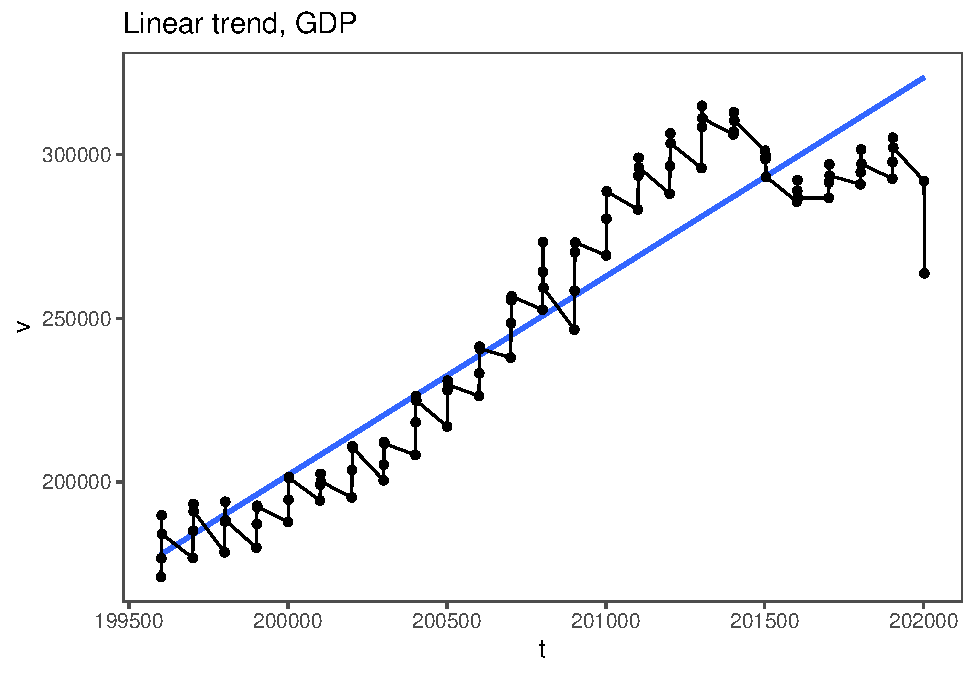
\includegraphics{Econo2_P5_files/figure-latex/parametric linear-1} \end{center}

Another way to find \(f_t\) is via a \emph{non-parametric} process. For
this, we'll use an HP filter and a moving average.

\begin{Shaded}
\begin{Highlighting}[]
\NormalTok{pib_ts <-}\StringTok{ }\KeywordTok{ts}\NormalTok{(pib}\OperatorTok{$}\NormalTok{v)}

\NormalTok{hp_trend <-}\StringTok{ }\KeywordTok{hpfilter}\NormalTok{(pib_ts, }\DataTypeTok{freq =} \DecValTok{1600}\NormalTok{, }\DataTypeTok{type =} \StringTok{"lambda"}\NormalTok{)}

\KeywordTok{plot}\NormalTok{(hp_trend)}
\end{Highlighting}
\end{Shaded}

\begin{center}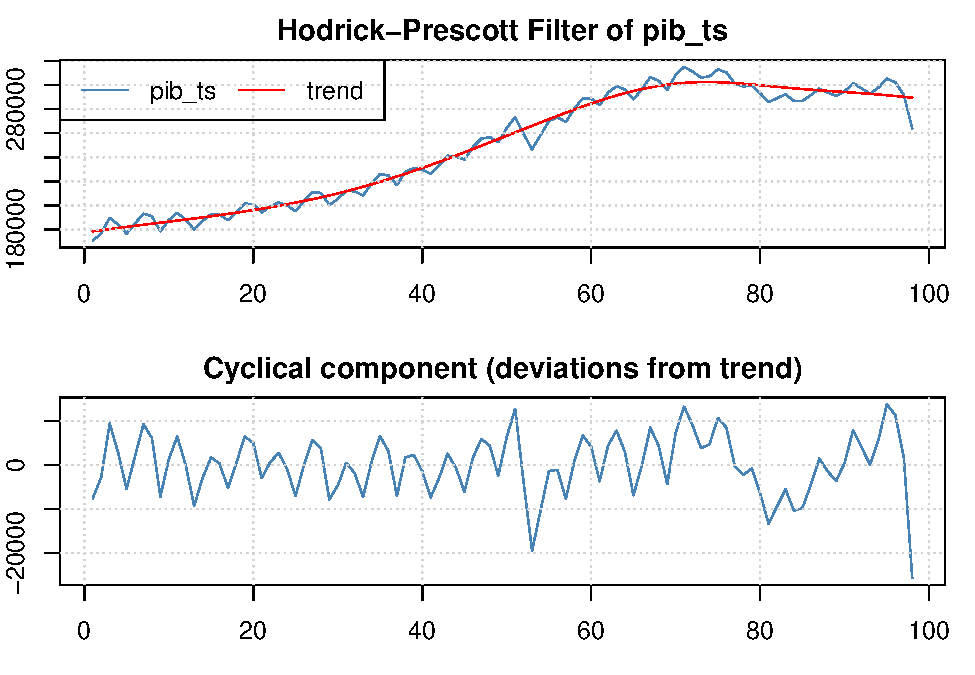
\includegraphics{Econo2_P5_files/figure-latex/hp filter-1} \end{center}

Now, a moving average.

\begin{Shaded}
\begin{Highlighting}[]
\NormalTok{pib_ma <-}\StringTok{ }\KeywordTok{ma}\NormalTok{(pib}\OperatorTok{$}\NormalTok{v, }\DataTypeTok{order =} \DecValTok{4}\NormalTok{)}

\KeywordTok{autoplot}\NormalTok{(pib_ma, }\DataTypeTok{color =} \StringTok{"blue"}\NormalTok{) }\OperatorTok{+}\StringTok{ }\KeywordTok{geom_line}\NormalTok{(}\DataTypeTok{data =}\NormalTok{ pib, }\KeywordTok{aes}\NormalTok{(}\DataTypeTok{x =} \DecValTok{1}\OperatorTok{:}\KeywordTok{length}\NormalTok{(pib}\OperatorTok{$}\NormalTok{t), }
    \DataTypeTok{y =}\NormalTok{ v), }\DataTypeTok{color =} \StringTok{"red"}\NormalTok{) }\OperatorTok{+}\StringTok{ }\KeywordTok{theme_few}\NormalTok{()}
\end{Highlighting}
\end{Shaded}

\begin{verbatim}
## Warning: Use of `pib$t` is discouraged. Use `t` instead.
\end{verbatim}

\begin{verbatim}
## Warning: Removed 4 row(s) containing missing values (geom_path).
\end{verbatim}

\begin{center}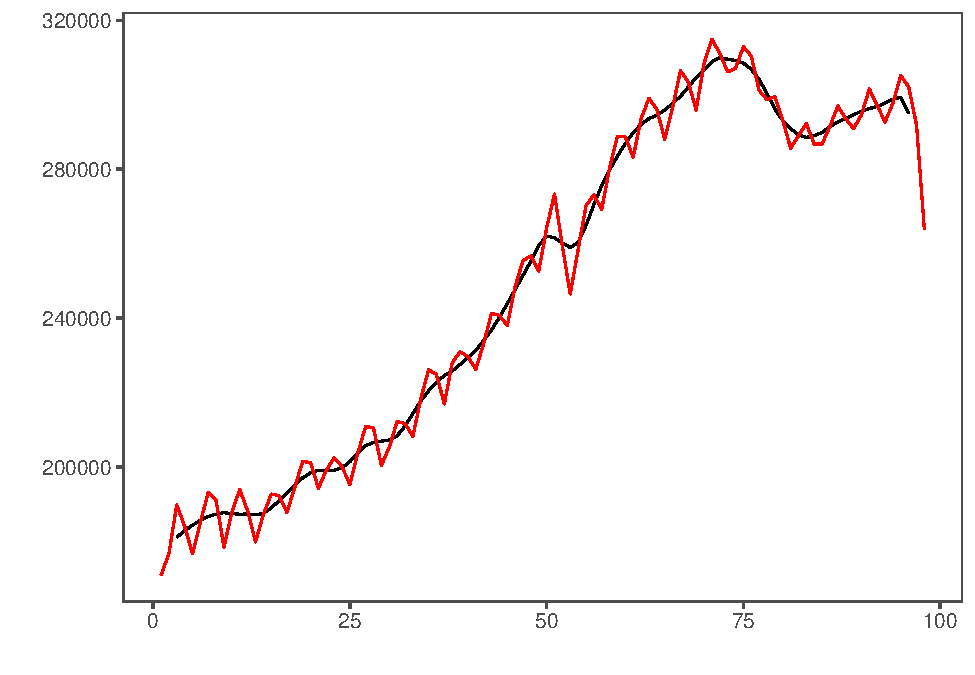
\includegraphics{Econo2_P5_files/figure-latex/moving average-1} \end{center}

\subsection{Seasonality}

We can now create a function for \(s_t\). This will be done with
dummies: \[ D_i = 1, i = t \] \[ D_i = 0 \, otherwise\]

\begin{Shaded}
\begin{Highlighting}[]
\NormalTok{tri <-}\StringTok{ }\KeywordTok{c}\NormalTok{(}\OtherTok{NA}\NormalTok{)}

\NormalTok{tri1 <-}\StringTok{ }\KeywordTok{c}\NormalTok{(}\DecValTok{1}\NormalTok{, }\DecValTok{2}\NormalTok{, }\DecValTok{3}\NormalTok{, }\DecValTok{4}\NormalTok{)}

\NormalTok{i =}\StringTok{ }\DecValTok{1}

\ControlFlowTok{while}\NormalTok{ (i }\OperatorTok{<}\StringTok{ }\DecValTok{25}\NormalTok{) \{}
    
\NormalTok{    tri <-}\StringTok{ }\KeywordTok{append}\NormalTok{(tri, tri1)}
    
\NormalTok{    i =}\StringTok{ }\NormalTok{i }\OperatorTok{+}\StringTok{ }\DecValTok{1}
    
\NormalTok{\}}

\NormalTok{tri <-}\StringTok{ }\NormalTok{tri[}\OperatorTok{-}\DecValTok{1}\NormalTok{]}
\NormalTok{tri <-}\StringTok{ }\KeywordTok{c}\NormalTok{(tri, }\DecValTok{1}\NormalTok{, }\DecValTok{2}\NormalTok{)}

\KeywordTok{length}\NormalTok{(tri)}
\end{Highlighting}
\end{Shaded}

\begin{verbatim}
## [1] 98
\end{verbatim}

\begin{Shaded}
\begin{Highlighting}[]
\NormalTok{pib <-}\StringTok{ }\KeywordTok{data.frame}\NormalTok{(pib, tri)}

\KeywordTok{names}\NormalTok{(pib)[}\DecValTok{1}\NormalTok{] <-}\StringTok{ "t"}
\KeywordTok{names}\NormalTok{(pib)[}\DecValTok{2}\NormalTok{] <-}\StringTok{ "v"}
\KeywordTok{names}\NormalTok{(pib)[}\DecValTok{3}\NormalTok{] <-}\StringTok{ "tri"}

\NormalTok{dummies <-}\StringTok{ }\KeywordTok{data.frame}\NormalTok{(}\KeywordTok{matrix}\NormalTok{(}\OtherTok{NA}\NormalTok{, }\DataTypeTok{nrow =} \KeywordTok{length}\NormalTok{(pib}\OperatorTok{$}\NormalTok{t), }\DataTypeTok{ncol =} \DecValTok{4}\NormalTok{))}

\ControlFlowTok{for}\NormalTok{ (j }\ControlFlowTok{in} \DecValTok{1}\OperatorTok{:}\DecValTok{4}\NormalTok{) \{}
    
\NormalTok{    dummies[j] <-}\StringTok{ }\KeywordTok{as.numeric}\NormalTok{(pib}\OperatorTok{$}\NormalTok{tri }\OperatorTok{==}\StringTok{ }\NormalTok{j)}
    
\NormalTok{\}}

\NormalTok{hp_fitted <-}\StringTok{ }\NormalTok{hp_trend[}\DecValTok{2}\NormalTok{]}

\NormalTok{hp_fitted <-}\StringTok{ }\NormalTok{hp_fitted}\OperatorTok{$}\NormalTok{trend}

\NormalTok{detrend <-}\StringTok{ }\NormalTok{pib}\OperatorTok{$}\NormalTok{v }\OperatorTok{-}\StringTok{ }\NormalTok{hp_fitted}

\NormalTok{pib <-}\StringTok{ }\KeywordTok{data.frame}\NormalTok{(pib, dummies, detrend)}

\KeywordTok{names}\NormalTok{(pib) <-}\StringTok{ }\KeywordTok{c}\NormalTok{(}\StringTok{"t"}\NormalTok{, }\StringTok{"v"}\NormalTok{, }\StringTok{"tri"}\NormalTok{, }\StringTok{"X1"}\NormalTok{, }\StringTok{"X2"}\NormalTok{, }\StringTok{"X3"}\NormalTok{, }\StringTok{"X4"}\NormalTok{, }\StringTok{"detrend"}\NormalTok{)}

\KeywordTok{head}\NormalTok{(pib)}
\end{Highlighting}
\end{Shaded}

\begin{verbatim}
##          t        v tri X1 X2 X3 X4   detrend
## 18  199601 170920.0   1  1  0  0  0 -7639.363
## 40  199602 176708.8   2  0  1  0  0 -2784.369
## 62  199603 189844.3   3  0  0  1  0  9422.159
## 84  199604 184112.9   4  0  0  0  1  2773.147
## 106 199701 176732.2   1  1  0  0  0 -5513.319
## 128 199702 185109.5   2  0  1  0  0  1968.942
\end{verbatim}

\begin{Shaded}
\begin{Highlighting}[]
\NormalTok{dummy_lm <-}\StringTok{ }\KeywordTok{lm}\NormalTok{(detrend }\OperatorTok{~}\StringTok{ }\NormalTok{X2 }\OperatorTok{+}\StringTok{ }\NormalTok{X3 }\OperatorTok{+}\StringTok{ }\NormalTok{X4, }\DataTypeTok{data =}\NormalTok{ pib)}

\KeywordTok{summary}\NormalTok{(dummy_lm)}
\end{Highlighting}
\end{Shaded}

\begin{verbatim}
## 
## Call:
## lm(formula = detrend ~ X2 + X3 + X4, data = pib)
## 
## Residuals:
##      Min       1Q   Median       3Q      Max 
## -24604.3  -2770.1    904.6   2781.6   9672.2 
## 
## Coefficients:
##             Estimate Std. Error t value Pr(>|t|)    
## (Intercept)    -5885       1079  -5.454 3.97e-07 ***
## X2              4775       1526   3.129  0.00234 ** 
## X3             11476       1542   7.443 4.63e-11 ***
## X4              7580       1542   4.916 3.73e-06 ***
## ---
## Signif. codes:  0 '***' 0.001 '**' 0.01 '*' 0.05 '.' 0.1 ' ' 1
## 
## Residual standard error: 5396 on 94 degrees of freedom
## Multiple R-squared:  0.3854, Adjusted R-squared:  0.3658 
## F-statistic: 19.65 on 3 and 94 DF,  p-value: 5.704e-10
\end{verbatim}

\subsection{$Y_t$}

We'll now use the HP-fitered version of \(f_t\) and the dummy approach
to \(s_t\).

\begin{Shaded}
\begin{Highlighting}[]
\NormalTok{yt <-}\StringTok{ }\KeywordTok{as.vector}\NormalTok{(pib}\OperatorTok{$}\NormalTok{v) }\OperatorTok{-}\StringTok{ }\NormalTok{(hp_fitted }\OperatorTok{+}\StringTok{ }\NormalTok{dummy_lm}\OperatorTok{$}\NormalTok{fitted.values)}

\KeywordTok{mean}\NormalTok{(yt)}
\end{Highlighting}
\end{Shaded}

\begin{verbatim}
## [1] 2.970866e-13
\end{verbatim}

\begin{Shaded}
\begin{Highlighting}[]
\KeywordTok{autoplot}\NormalTok{(yt) }\OperatorTok{+}\StringTok{ }\KeywordTok{theme_few}\NormalTok{()}
\end{Highlighting}
\end{Shaded}

\begin{center}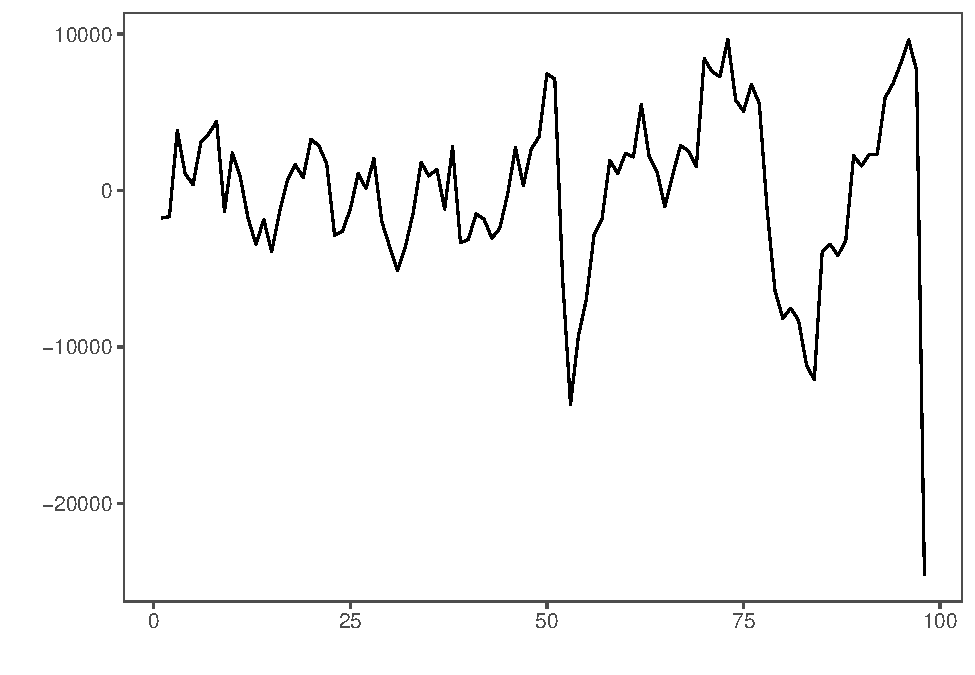
\includegraphics{Econo2_P5_files/figure-latex/stochastic yt-1} \end{center}

\begin{Shaded}
\begin{Highlighting}[]
\NormalTok{y <-}\StringTok{ }\KeywordTok{data.frame}\NormalTok{(}\DecValTok{1}\OperatorTok{:}\DecValTok{98}\NormalTok{, yt)}

\KeywordTok{names}\NormalTok{(y) <-}\StringTok{ }\KeywordTok{c}\NormalTok{(}\StringTok{"t"}\NormalTok{, }\StringTok{"yt"}\NormalTok{)}

\NormalTok{y}
\end{Highlighting}
\end{Shaded}

\begin{verbatim}
##     t          yt
## 1   1  -1754.3235
## 2   2  -1674.2366
## 3   3   3831.0260
## 4   4   1077.6423
## 5   5    371.7207
## 6   6   3079.0752
## 7   7   3631.4076
## 8   8   4410.6091
## 9   9  -1349.8941
## 10 10   2409.3970
## 11 11    876.5449
## 12 12  -1771.0299
## 13 13  -3446.9097
## 14 14  -1862.9712
## 15 15  -3915.0963
## 16 16  -1385.6491
## 17 17    660.2786
## 18 18   1651.6795
## 19 19    825.0142
## 20 20   3270.0845
## 21 21   2865.9816
## 22 22   1715.7519
## 23 23  -2863.5994
## 24 24  -2593.0754
## 25 25  -1198.5249
## 26 26   1080.3232
## 27 27    137.0892
## 28 28   2050.1420
## 29 29  -1969.7004
## 30 30  -3594.0722
## 31 31  -5112.3766
## 32 32  -3600.7764
## 33 33  -1415.4644
## 34 34   1805.2058
## 35 35    932.6659
## 36 36   1357.1028
## 37 37  -1188.4845
## 38 38   2797.7938
## 39 39  -3335.8195
## 40 40  -3130.3567
## 41 41  -1492.3199
## 42 42  -1837.9660
## 43 43  -3043.8690
## 44 44  -2423.6004
## 45 45   -245.9843
## 46 46   2733.1889
## 47 47    312.7526
## 48 48   2649.9160
## 49 49   3436.5474
## 50 50   7473.7381
## 51 51   7140.3317
## 52 52  -5705.3555
## 53 53 -13671.1151
## 54 54  -9312.6039
## 55 55  -6991.8338
## 56 56  -2829.1628
## 57 57  -1842.3440
## 58 58   1936.3965
## 59 59   1088.5846
## 60 60   2385.4095
## 61 61   2147.8149
## 62 62   5521.2927
## 63 63   2177.2726
## 64 64   1198.7473
## 65 65  -1037.2566
## 66 66   1022.4375
## 67 67   2879.2346
## 68 68   2522.7543
## 69 69   1511.4818
## 70 70   8425.6844
## 71 71   7607.8450
## 72 72   7279.1542
## 73 73   9672.2025
## 74 74   5783.3700
## 75 75   5071.2219
## 76 76   6770.3224
## 77 77   5577.1514
## 78 78  -1208.9140
## 79 79  -6401.7422
## 80 80  -8180.8921
## 81 81  -7524.9466
## 82 82  -8309.2567
## 83 83 -11139.4502
## 84 84 -12109.4675
## 85 85  -3944.6523
## 86 86  -3427.1807
## 87 87  -4155.8533
## 88 88  -3196.0049
## 89 89   2214.9221
## 90 90   1569.5815
## 91 91   2315.4632
## 92 92   2322.1098
## 93 93   5932.3518
## 94 94   6826.5670
## 95 95   8133.1861
## 96 96   9631.3765
## 97 97   7691.4677
## 98 98 -24604.2816
\end{verbatim}

\section{Identifying and estimating ARMA(p,q) for $Y_t$}

We are now in a position to identify and estimate the best model for our
time series \(Y_t\).

Applying the function \emph{auto.arima} from the package \emph{forecast}
to identify and estimate the model:

\begin{Shaded}
\begin{Highlighting}[]
\NormalTok{aa_model <-}\StringTok{ }\KeywordTok{auto.arima}\NormalTok{(y}\OperatorTok{$}\NormalTok{yt, }\DataTypeTok{num.cores =} \DecValTok{24}\NormalTok{, }\DataTypeTok{max.d =} \DecValTok{0}\NormalTok{, }\DataTypeTok{stepwise =}\NormalTok{ F)}

\KeywordTok{summary}\NormalTok{(aa_model)}
\end{Highlighting}
\end{Shaded}

\begin{verbatim}
## Series: y$yt 
## ARIMA(2,0,2) with zero mean 
## 
## Coefficients:
##           ar1     ar2     ma1     ma2
##       -0.5799  0.3799  1.6394  0.7070
## s.e.   0.1463  0.1453  0.1191  0.1165
## 
## sigma^2 estimated as 16014834:  log likelihood=-951.01
## AIC=1912.01   AICc=1912.66   BIC=1924.94
## 
## Training set error measures:
##                     ME     RMSE      MAE      MPE     MAPE      MASE
## Training set -166.6391 3919.333 2469.197 32.42135 93.29931 0.9554301
##                      ACF1
## Training set -0.001381943
\end{verbatim}

\begin{Shaded}
\begin{Highlighting}[]
\KeywordTok{print}\NormalTok{(}\StringTok{"t-values: "}\NormalTok{)}
\end{Highlighting}
\end{Shaded}

\begin{verbatim}
## [1] "t-values: "
\end{verbatim}

\begin{Shaded}
\begin{Highlighting}[]
\NormalTok{aa_t <-}\StringTok{ }\KeywordTok{matrix}\NormalTok{(}\OtherTok{NA}\NormalTok{, }\DataTypeTok{nrow =}\NormalTok{ aa_model}\OperatorTok{$}\NormalTok{arma[}\DecValTok{1}\NormalTok{] }\OperatorTok{+}\StringTok{ }\NormalTok{aa_model}\OperatorTok{$}\NormalTok{arma[}\DecValTok{2}\NormalTok{])}

\ControlFlowTok{for}\NormalTok{ (i }\ControlFlowTok{in} \KeywordTok{c}\NormalTok{(}\DecValTok{1}\OperatorTok{:}\NormalTok{(aa_model}\OperatorTok{$}\NormalTok{arma[}\DecValTok{1}\NormalTok{] }\OperatorTok{+}\StringTok{ }\NormalTok{aa_model}\OperatorTok{$}\NormalTok{arma[}\DecValTok{2}\NormalTok{]))) \{}
    
\NormalTok{    aa_t[i] <-}\StringTok{ }\NormalTok{aa_model}\OperatorTok{$}\NormalTok{coef[i]}\OperatorTok{/}\KeywordTok{sqrt}\NormalTok{(aa_model}\OperatorTok{$}\NormalTok{var.coef[i, i])}
    
\NormalTok{\}}

\NormalTok{aa_t <-}\StringTok{ }\KeywordTok{data.frame}\NormalTok{(aa_t)}

\NormalTok{aa_t}
\end{Highlighting}
\end{Shaded}

\begin{verbatim}
##        aa_t
## 1 -3.965137
## 2  2.614792
## 3 13.768478
## 4  6.067555
\end{verbatim}

\begin{Shaded}
\begin{Highlighting}[]
\NormalTok{aa_q <-}\StringTok{ }\KeywordTok{Box.test}\NormalTok{(aa_model}\OperatorTok{$}\NormalTok{residuals, }\DataTypeTok{lag =}\NormalTok{ aa_model}\OperatorTok{$}\NormalTok{arma[}\DecValTok{1}\NormalTok{] }\OperatorTok{+}\StringTok{ }
\StringTok{    }\NormalTok{aa_model}\OperatorTok{$}\NormalTok{arma[}\DecValTok{2}\NormalTok{])}
\NormalTok{aa_q}
\end{Highlighting}
\end{Shaded}

\begin{verbatim}
## 
##  Box-Pierce test
## 
## data:  aa_model$residuals
## X-squared = 0.22, df = 4, p-value = 0.9944
\end{verbatim}

\begin{Shaded}
\begin{Highlighting}[]
\NormalTok{criteria <-}\StringTok{ }\KeywordTok{matrix}\NormalTok{(}\OtherTok{NA}\NormalTok{, }\DataTypeTok{nrow =} \DecValTok{1}\NormalTok{, }\DataTypeTok{ncol =} \DecValTok{3}\NormalTok{)}

\NormalTok{aa_criteria <-}\StringTok{ }\KeywordTok{data.frame}\NormalTok{(}\StringTok{"AR(2)*"}\NormalTok{, aa_model}\OperatorTok{$}\NormalTok{aic, aa_model}\OperatorTok{$}\NormalTok{bic)}

\KeywordTok{names}\NormalTok{(aa_criteria) <-}\StringTok{ }\KeywordTok{c}\NormalTok{(}\StringTok{"Model"}\NormalTok{, }\StringTok{"AIC"}\NormalTok{, }\StringTok{"BIC"}\NormalTok{)}

\NormalTok{aa_criteria}
\end{Highlighting}
\end{Shaded}

\begin{verbatim}
##    Model      AIC      BIC
## 1 AR(2)* 1912.011 1924.936
\end{verbatim}

\begin{Shaded}
\begin{Highlighting}[]
\NormalTok{fac_e <-}\StringTok{ }\KeywordTok{ggAcf}\NormalTok{(aa_model}\OperatorTok{$}\NormalTok{residuals, }\DataTypeTok{type =} \StringTok{"correlation"}\NormalTok{, }\DataTypeTok{lag.max =} \DecValTok{30}\NormalTok{, }
    \DataTypeTok{plot =}\NormalTok{ T) }\OperatorTok{+}\StringTok{ }\KeywordTok{theme_few}\NormalTok{()}

\NormalTok{facp_e <-}\StringTok{ }\KeywordTok{ggPacf}\NormalTok{(aa_model}\OperatorTok{$}\NormalTok{residuals, }\DataTypeTok{type =} \StringTok{"correlation"}\NormalTok{, }\DataTypeTok{lag.max =} \DecValTok{30}\NormalTok{, }
    \DataTypeTok{plot =}\NormalTok{ T) }\OperatorTok{+}\StringTok{ }\KeywordTok{theme_few}\NormalTok{()}
\end{Highlighting}
\end{Shaded}

\begin{verbatim}
## Warning: Ignoring unknown parameters: type
\end{verbatim}

\begin{Shaded}
\begin{Highlighting}[]
\NormalTok{fac_e}
\end{Highlighting}
\end{Shaded}

\begin{center}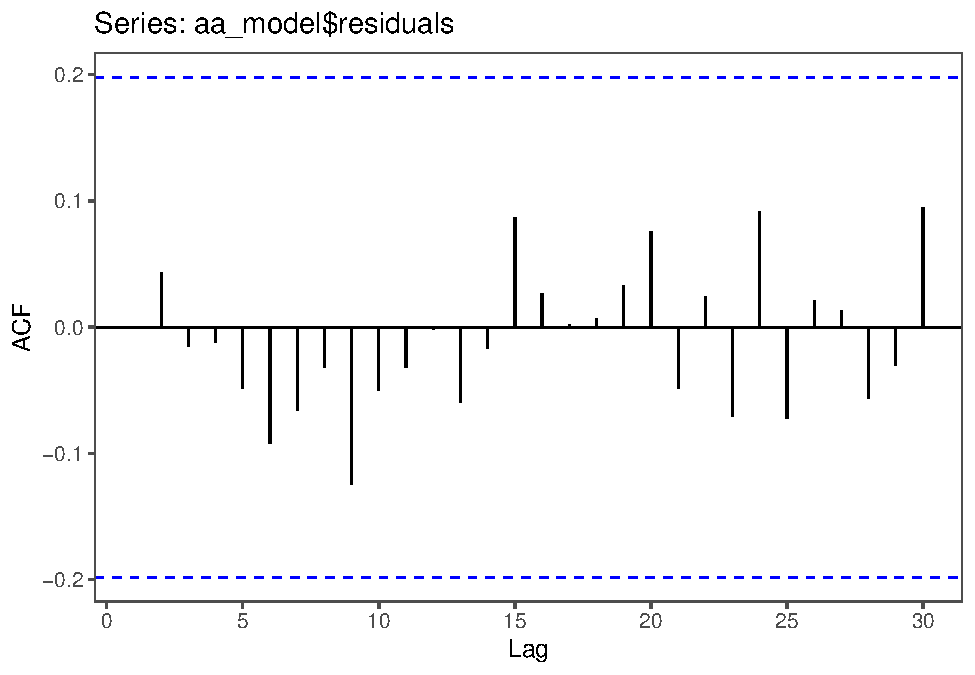
\includegraphics{Econo2_P5_files/figure-latex/estimation autoarima-1} \end{center}

\begin{Shaded}
\begin{Highlighting}[]
\NormalTok{facp_e}
\end{Highlighting}
\end{Shaded}

\begin{center}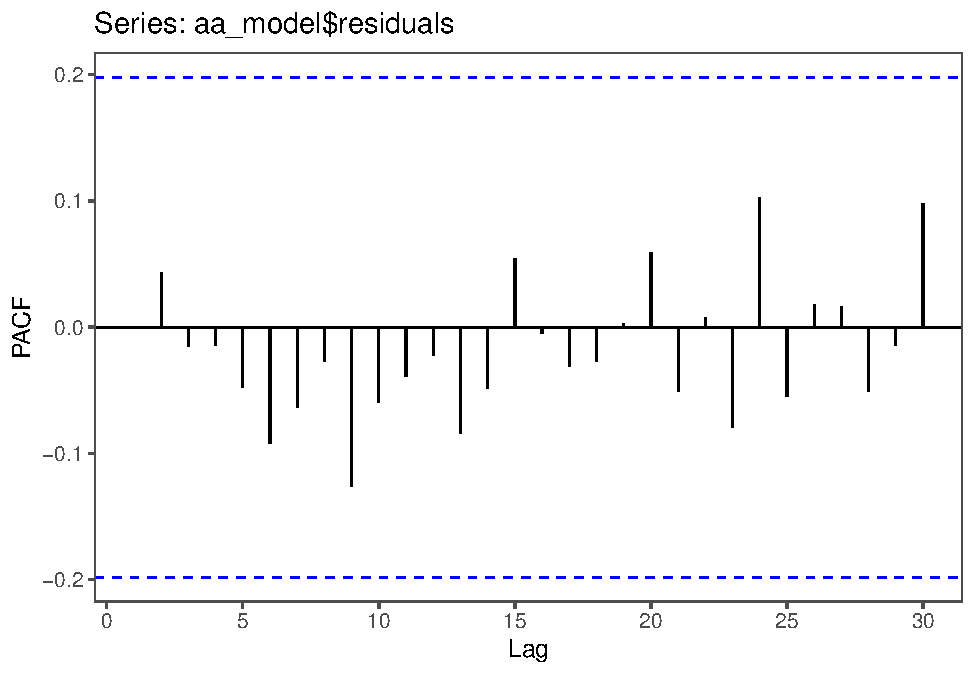
\includegraphics{Econo2_P5_files/figure-latex/estimation autoarima-2} \end{center}

\begin{Shaded}
\begin{Highlighting}[]
\KeywordTok{mean}\NormalTok{(aa_model}\OperatorTok{$}\NormalTok{residuals)}
\end{Highlighting}
\end{Shaded}

\begin{verbatim}
## [1] -166.6391
\end{verbatim}

\begin{Shaded}
\begin{Highlighting}[]
\KeywordTok{plot}\NormalTok{(aa_model}\OperatorTok{$}\NormalTok{residuals)}
\end{Highlighting}
\end{Shaded}

\begin{center}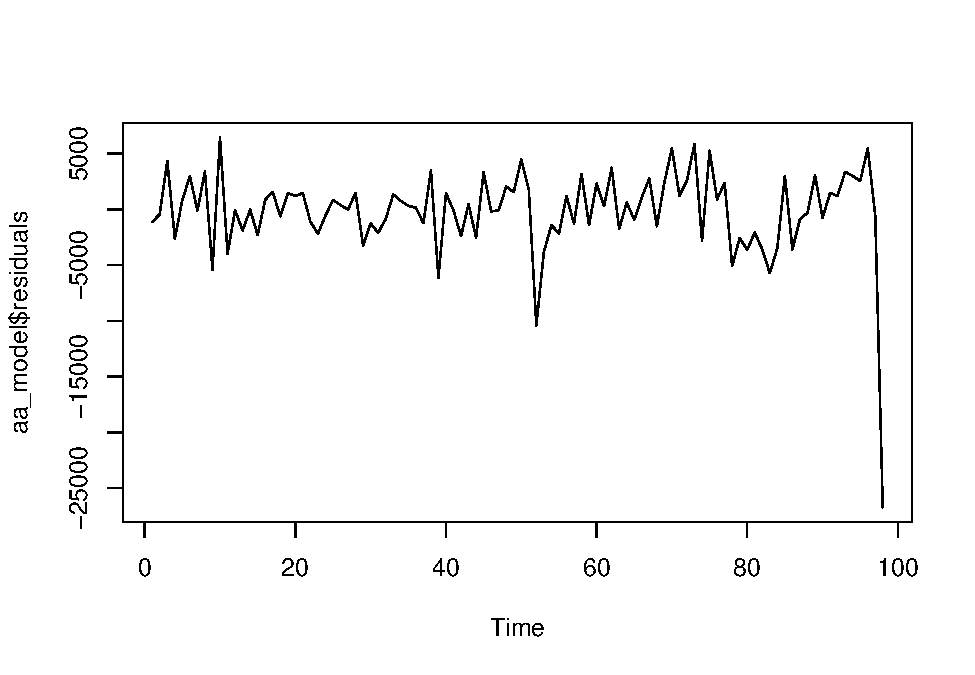
\includegraphics{Econo2_P5_files/figure-latex/estimation autoarima-3} \end{center}

\begin{Shaded}
\begin{Highlighting}[]
\NormalTok{facst <-}\StringTok{ }\KeywordTok{ggAcf}\NormalTok{(y}\OperatorTok{$}\NormalTok{yt, }\DataTypeTok{type =} \StringTok{"correlation"}\NormalTok{, }\DataTypeTok{lag.max =} \DecValTok{30}\NormalTok{, }\DataTypeTok{plot =}\NormalTok{ T) }\OperatorTok{+}\StringTok{ }
\StringTok{    }\KeywordTok{theme_few}\NormalTok{()}
\NormalTok{faclt <-}\StringTok{ }\KeywordTok{ggAcf}\NormalTok{(y}\OperatorTok{$}\NormalTok{yt, }\DataTypeTok{type =} \StringTok{"correlation"}\NormalTok{, }\DataTypeTok{lag.max =} \DecValTok{5000}\NormalTok{, }\DataTypeTok{plot =}\NormalTok{ T) }\OperatorTok{+}\StringTok{ }
\StringTok{    }\KeywordTok{theme_few}\NormalTok{()}

\NormalTok{facpst <-}\StringTok{ }\KeywordTok{ggPacf}\NormalTok{(y}\OperatorTok{$}\NormalTok{yt, }\DataTypeTok{type =} \StringTok{"correlation"}\NormalTok{, }\DataTypeTok{lag.max =} \DecValTok{30}\NormalTok{, }\DataTypeTok{plot =}\NormalTok{ T) }\OperatorTok{+}\StringTok{ }
\StringTok{    }\KeywordTok{theme_few}\NormalTok{()}
\end{Highlighting}
\end{Shaded}

\begin{verbatim}
## Warning: Ignoring unknown parameters: type
\end{verbatim}

\begin{Shaded}
\begin{Highlighting}[]
\NormalTok{facplt <-}\StringTok{ }\KeywordTok{ggPacf}\NormalTok{(y}\OperatorTok{$}\NormalTok{yt, }\DataTypeTok{type =} \StringTok{"correlation"}\NormalTok{, }\DataTypeTok{lag.max =} \DecValTok{5000}\NormalTok{, }
    \DataTypeTok{plot =}\NormalTok{ T) }\OperatorTok{+}\StringTok{ }\KeywordTok{theme_few}\NormalTok{()}
\end{Highlighting}
\end{Shaded}

\begin{verbatim}
## Warning: Ignoring unknown parameters: type
\end{verbatim}

\begin{Shaded}
\begin{Highlighting}[]
\NormalTok{facst}
\end{Highlighting}
\end{Shaded}

\begin{center}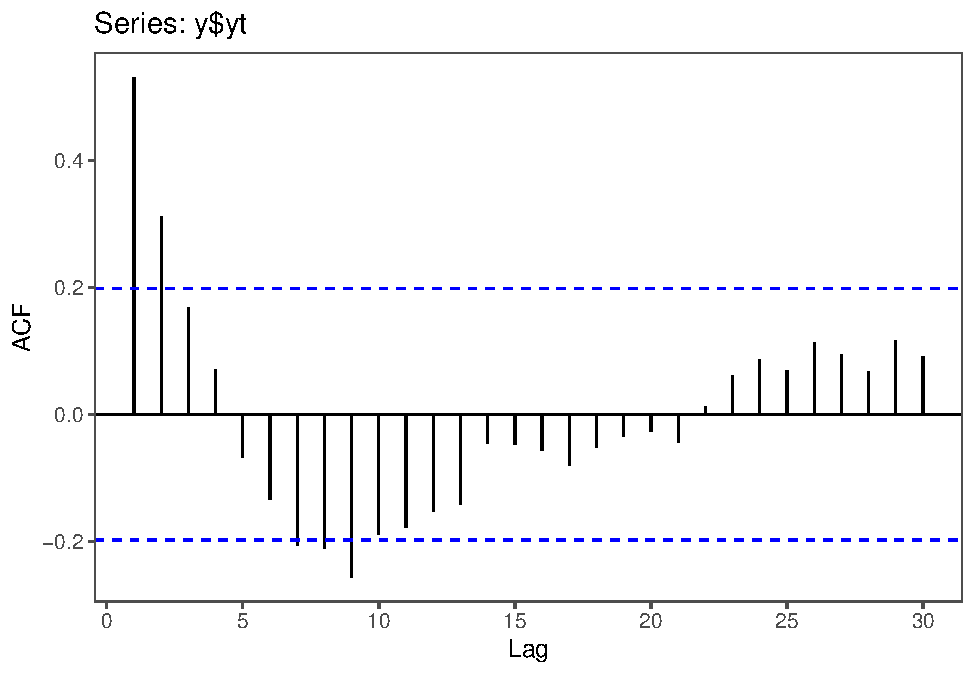
\includegraphics{Econo2_P5_files/figure-latex/plots fac facp-1} \end{center}

\begin{Shaded}
\begin{Highlighting}[]
\NormalTok{faclt}
\end{Highlighting}
\end{Shaded}

\begin{center}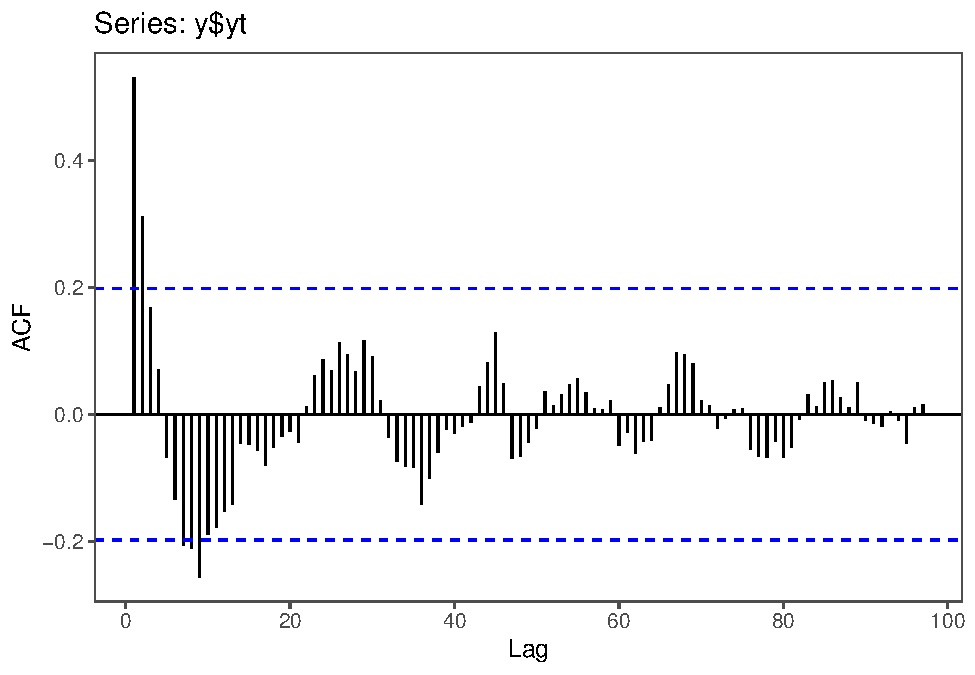
\includegraphics{Econo2_P5_files/figure-latex/plots fac facp-2} \end{center}

\begin{Shaded}
\begin{Highlighting}[]
\NormalTok{facpst}
\end{Highlighting}
\end{Shaded}

\begin{center}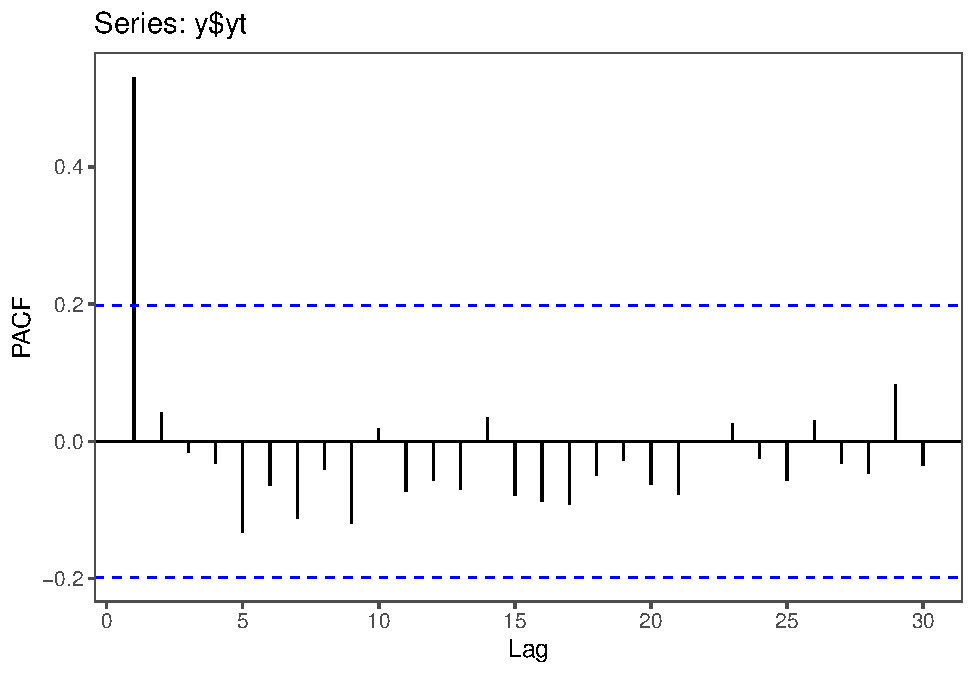
\includegraphics{Econo2_P5_files/figure-latex/plots fac facp-3} \end{center}

\begin{Shaded}
\begin{Highlighting}[]
\NormalTok{facplt}
\end{Highlighting}
\end{Shaded}

\begin{center}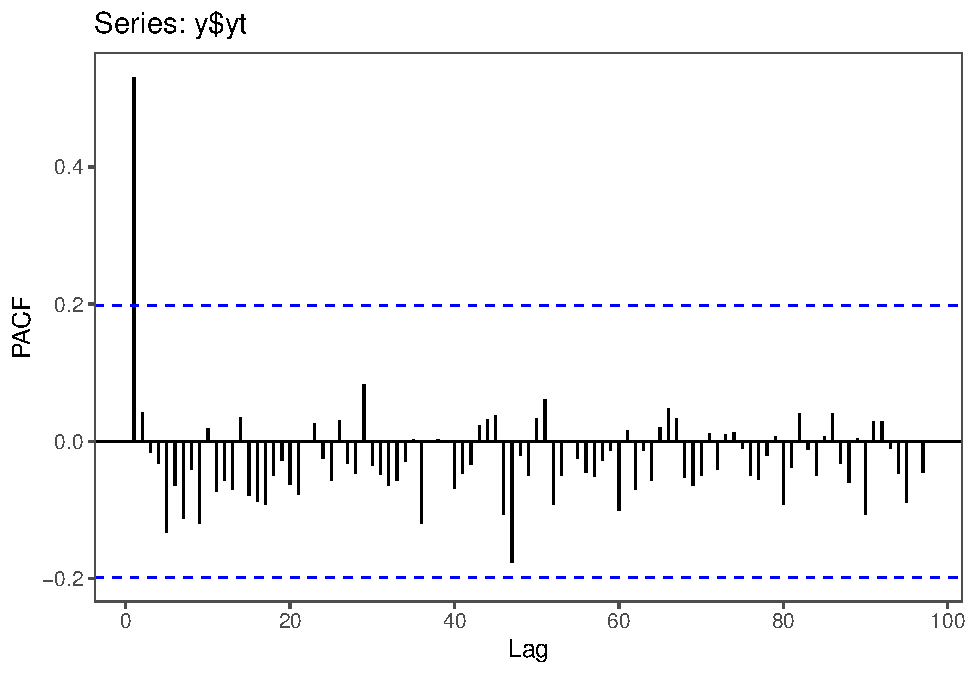
\includegraphics{Econo2_P5_files/figure-latex/plots fac facp-4} \end{center}

The results of \emph{auto.arima} imply that the best model is an
ARMA(2,0) -- i.e., an AR(2):
\[ y_t = c + \phi_1 y_{t-1} + \phi_2 y_{t-2} + \varepsilon_t, \hspace{1em} \varepsilon_t \sim wn(0, \sigma^2)\]

\begin{Shaded}
\begin{Highlighting}[]
\NormalTok{fc <-}\StringTok{ }\KeywordTok{forecast}\NormalTok{(y}\OperatorTok{$}\NormalTok{yt, }\DataTypeTok{model =}\NormalTok{ aa_model, }\DataTypeTok{h =} \DecValTok{4}\NormalTok{)}

\KeywordTok{autoplot}\NormalTok{(fc) }\OperatorTok{+}\StringTok{ }\KeywordTok{theme_few}\NormalTok{()}
\end{Highlighting}
\end{Shaded}

\begin{verbatim}
## Warning: `filter_()` is deprecated as of dplyr 0.7.0.
## Please use `filter()` instead.
## See vignette('programming') for more help
## This warning is displayed once every 8 hours.
## Call `lifecycle::last_warnings()` to see where this warning was generated.
\end{verbatim}

\begin{center}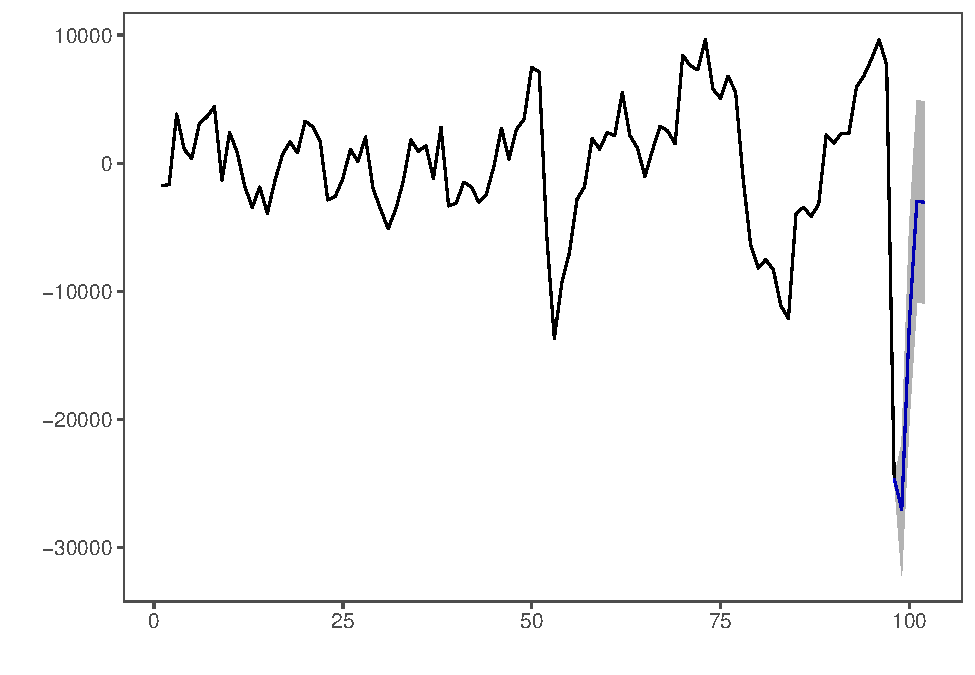
\includegraphics{Econo2_P5_files/figure-latex/forecast plot-1} \end{center}

\section{Long term GDP growth}

\begin{Shaded}
\begin{Highlighting}[]
\NormalTok{unemp <-}\StringTok{ }\KeywordTok{read_excel}\NormalTok{(}\StringTok{"C:/Users/William/Downloads/tabela2176.xlsx"}\NormalTok{)}
\end{Highlighting}
\end{Shaded}

\begin{verbatim}
## New names:
## * `` -> ...2
## * `` -> ...3
## * `` -> ...4
## * `` -> ...5
## * `` -> ...6
## * ...
\end{verbatim}

\begin{Shaded}
\begin{Highlighting}[]
\NormalTok{unemp1 <-}\StringTok{ }\KeywordTok{as.numeric}\NormalTok{(unemp[}\DecValTok{11}\NormalTok{, ])}
\end{Highlighting}
\end{Shaded}

\begin{verbatim}
## Warning: NAs introduced by coercion
\end{verbatim}

\begin{Shaded}
\begin{Highlighting}[]
\NormalTok{unemp2 <-}\StringTok{ }\NormalTok{unemp1[}\DecValTok{2}\OperatorTok{:}\NormalTok{(}\KeywordTok{length}\NormalTok{(unemp1) }\OperatorTok{-}\StringTok{ }\DecValTok{2}\NormalTok{)]}

\NormalTok{unemp <-}\StringTok{ }\NormalTok{unemp2}

\NormalTok{df_unemp <-}\StringTok{ }\KeywordTok{data.frame}\NormalTok{(}\DecValTok{1}\OperatorTok{:}\KeywordTok{length}\NormalTok{(unemp), unemp)}

\KeywordTok{names}\NormalTok{(df_unemp) <-}\StringTok{ }\KeywordTok{c}\NormalTok{(}\StringTok{"t"}\NormalTok{, }\StringTok{"r"}\NormalTok{)}

\NormalTok{df_unemp}
\end{Highlighting}
\end{Shaded}

\begin{verbatim}
##       t    r
## 1     1 12.9
## 2     2 12.5
## 3     3 11.9
## 4     4 11.6
## 5     5 11.9
## 6     6 11.7
## 7     7 11.5
## 8     8 11.2
## 9     9 10.9
## 10   10 10.5
## 11   11 11.2
## 12   12 11.6
## 13   13 12.1
## 14   14 12.4
## 15   15 12.9
## 16   16 13.0
## 17   17 12.8
## 18   18 13.0
## 19   19 13.0
## 20   20 12.9
## 21   21 12.2
## 22   22 10.9
## 23   23 11.7
## 24   24 12.0
## 25   25 12.8
## 26   26 13.1
## 27   27 12.2
## 28   28 11.7
## 29   29 11.2
## 30   30 11.4
## 31   31 10.9
## 32   32 10.5
## 33   33 10.7
## 34   34  9.6
## 35   35 10.2
## 36   36 10.7
## 37   37 10.8
## 38   38 10.8
## 39   39 10.2
## 40   40  9.4
## 41   41  9.4
## 42   42  9.4
## 43   43  9.6
## 44   44  9.6
## 45   45  9.6
## 46   46  8.4
## 47   47  9.3
## 48   48 10.1
## 49   49 10.4
## 50   50 10.4
## 51   51 10.2
## 52   52 10.4
## 53   53 10.7
## 54   54 10.6
## 55   55 10.0
## 56   56  9.8
## 57   57  9.5
## 58   58  8.4
## 59   59  9.3
## 60   60  9.9
## 61   61 10.2
## 62   62 10.2
## 63   63 10.2
## 64   64  9.7
## 65   65  9.5
## 66   66  9.5
## 67   67  9.0
## 68   68  8.7
## 69   69  8.2
## 70   70  7.4
## 71   71  8.0
## 72   72  8.7
## 73   73  8.6
## 74   74  8.5
## 75   75  7.9
## 76   76  7.8
## 77   77  8.1
## 78   78  7.6
## 79   79  7.7
## 80   80  7.5
## 81   81  7.6
## 82   82  6.8
## 83   83  8.2
## 84   84  8.5
## 85   85  9.0
## 86   86  8.9
## 87   87  8.8
## 88   88  8.1
## 89   89  8.0
## 90   90  8.1
## 91   91  7.7
## 92   92  7.5
## 93   93  7.3
## 94   94  6.8
## 95   95  7.2
## 96   96  7.4
## 97   97  7.6
## 98   98  7.3
## 99   99  7.4
## 100 100  7.0
## 101 101  6.9
## 102 102  6.7
## 103 103  6.2
## 104 104  6.0
## 105 105  5.7
## 106 106  5.3
## 107 107  6.0
## 108 108  6.3
## 109 109  6.4
## 110 110  6.4
## 111 111  6.3
## 112 112  6.2
## 113 113  6.0
## 114 114  6.0
## 115 115  6.0
## 116 116  5.7
## 117 117  5.2
## 118 118  4.7
## 119 119  5.5
## 120 120  5.7
## 121 121  6.2
## 122 122  6.0
## 123 123  5.8
## 124 124  5.9
## 125 125  5.4
## 126 126  5.3
## 127 127  5.4
## 128 128  5.3
## 129 129  4.9
## 130 130  4.6
## 131 131  5.5
## 132 132  5.6
## 133 133  5.7
## 134 134  5.8
## 135 135  5.8
## 136 136  6.0
## 137 137  5.6
## 138 138  5.3
## 139 139  5.4
## 140 140  5.2
## 141 141  4.6
## 142 142  4.3
## 143 143  4.8
## 144 144  5.1
## 145 145  5.0
## 146 146  4.8
## 147 147  4.9
## 148 148  4.8
## 149 149  4.9
## 150 150  5.0
## 151 151  4.8
## 152 152  4.6
## 153 153  4.8
## 154 154  4.3
## 155 155  5.3
## 156 156  5.8
## 157 157  6.1
## 158 158  6.4
## 159 159  6.7
## 160 160  6.9
## 161 161  7.5
## 162 162  7.5
## 163 163  7.5
## 164 164  7.8
## 165 165  7.5
## 166 166  6.9
\end{verbatim}

\begin{Shaded}
\begin{Highlighting}[]
\NormalTok{hp_unemp <-}\StringTok{ }\KeywordTok{hpfilter}\NormalTok{(df_unemp}\OperatorTok{$}\NormalTok{r, }\DataTypeTok{freq =} \DecValTok{1600}\NormalTok{, }\DataTypeTok{type =} \StringTok{"lambda"}\NormalTok{)}

\KeywordTok{plot}\NormalTok{(hp_unemp)}
\end{Highlighting}
\end{Shaded}

\begin{center}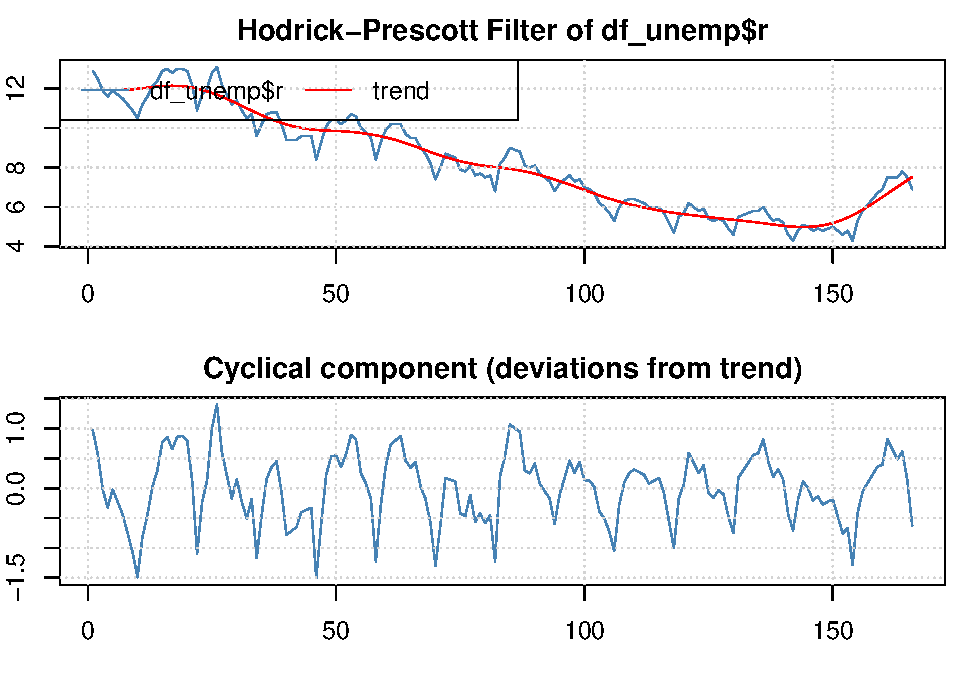
\includegraphics{Econo2_P5_files/figure-latex/loading data pme-1} \end{center}

\begin{Shaded}
\begin{Highlighting}[]
\NormalTok{nairu <-}\StringTok{ }\NormalTok{hp_unemp}\OperatorTok{$}\NormalTok{trend}

\NormalTok{nairu}
\end{Highlighting}
\end{Shaded}

\begin{verbatim}
##             [,1]
##   [1,] 11.927416
##   [2,] 11.924286
##   [3,] 11.921765
##   [4,] 11.920818
##   [5,] 11.922402
##   [6,] 11.927269
##   [7,] 11.936158
##   [8,] 11.949668
##   [9,] 11.968123
##  [10,] 11.991379
##  [11,] 12.018626
##  [12,] 12.048121
##  [13,] 12.077607
##  [14,] 12.104550
##  [15,] 12.126430
##  [16,] 12.140909
##  [17,] 12.146136
##  [18,] 12.140793
##  [19,] 12.123974
##  [20,] 12.095308
##  [21,] 12.054973
##  [22,] 12.003649
##  [23,] 11.942106
##  [24,] 11.870426
##  [25,] 11.788538
##  [26,] 11.696453
##  [27,] 11.594813
##  [28,] 11.485140
##  [29,] 11.369331
##  [30,] 11.249419
##  [31,] 11.127330
##  [32,] 11.005086
##  [33,] 10.884566
##  [34,] 10.767331
##  [35,] 10.654831
##  [36,] 10.547783
##  [37,] 10.446622
##  [38,] 10.351876
##  [39,] 10.264295
##  [40,] 10.184909
##  [41,] 10.114709
##  [42,] 10.054192
##  [43,] 10.003413
##  [44,]  9.962014
##  [45,]  9.929387
##  [46,]  9.904698
##  [47,]  9.886905
##  [48,]  9.874028
##  [49,]  9.863719
##  [50,]  9.853772
##  [51,]  9.842314
##  [52,]  9.827816
##  [53,]  9.808972
##  [54,]  9.784832
##  [55,]  9.755005
##  [56,]  9.719608
##  [57,]  9.678911
##  [58,]  9.633236
##  [59,]  9.582792
##  [60,]  9.527016
##  [61,]  9.465171
##  [62,]  9.396752
##  [63,]  9.321711
##  [64,]  9.240505
##  [65,]  9.154139
##  [66,]  9.063905
##  [67,]  8.971311
##  [68,]  8.878138
##  [69,]  8.786185
##  [70,]  8.697138
##  [71,]  8.612320
##  [72,]  8.532241
##  [73,]  8.457027
##  [74,]  8.386911
##  [75,]  8.322216
##  [76,]  8.263334
##  [77,]  8.210393
##  [78,]  8.163232
##  [79,]  8.121622
##  [80,]  8.084981
##  [81,]  8.052462
##  [82,]  8.022855
##  [83,]  7.994666
##  [84,]  7.965636
##  [85,]  7.933637
##  [86,]  7.896871
##  [87,]  7.854210
##  [88,]  7.805152
##  [89,]  7.749784
##  [90,]  7.688379
##  [91,]  7.621368
##  [92,]  7.549437
##  [93,]  7.473321
##  [94,]  7.393725
##  [95,]  7.311247
##  [96,]  7.226110
##  [97,]  7.138472
##  [98,]  7.048596
##  [99,]  6.957036
## [100,]  6.864503
## [101,]  6.771982
## [102,]  6.680546
## [103,]  6.591347
## [104,]  6.505548
## [105,]  6.424068
## [106,]  6.347512
## [107,]  6.276030
## [108,]  6.209117
## [109,]  6.146098
## [110,]  6.086352
## [111,]  6.029420
## [112,]  5.975035
## [113,]  5.923103
## [114,]  5.873667
## [115,]  5.826822
## [116,]  5.782738
## [117,]  5.741696
## [118,]  5.703924
## [119,]  5.669312
## [120,]  5.637122
## [121,]  5.606511
## [122,]  5.576675
## [123,]  5.547180
## [124,]  5.517857
## [125,]  5.488697
## [126,]  5.459926
## [127,]  5.431719
## [128,]  5.404147
## [129,]  5.377264
## [130,]  5.351057
## [131,]  5.325217
## [132,]  5.298963
## [133,]  5.271624
## [134,]  5.242719
## [135,]  5.212032
## [136,]  5.179698
## [137,]  5.146216
## [138,]  5.112602
## [139,]  5.080152
## [140,]  5.050281
## [141,]  5.024603
## [142,]  5.004827
## [143,]  4.992394
## [144,]  4.988308
## [145,]  4.993449
## [146,]  5.008769
## [147,]  5.035225
## [148,]  5.073642
## [149,]  5.124759
## [150,]  5.189148
## [151,]  5.267236
## [152,]  5.359336
## [153,]  5.465466
## [154,]  5.585171
## [155,]  5.717579
## [156,]  5.861015
## [157,]  6.013544
## [158,]  6.173192
## [159,]  6.338039
## [160,]  6.506307
## [161,]  6.676444
## [162,]  6.847145
## [163,]  7.017617
## [164,]  7.187480
## [165,]  7.356650
## [166,]  7.525429
\end{verbatim}

\begin{Shaded}
\begin{Highlighting}[]
\NormalTok{t6162 <-}\StringTok{ }\KeywordTok{get_sidra}\NormalTok{(}\DecValTok{6612}\NormalTok{, }\DataTypeTok{variable =} \DecValTok{9318}\NormalTok{, }\DataTypeTok{category =} \DecValTok{90707}\NormalTok{, }\DataTypeTok{period =} \KeywordTok{c}\NormalTok{(}\StringTok{"200202"}\NormalTok{, }
    \StringTok{"200203"}\NormalTok{, }\StringTok{"200204"}\NormalTok{, }\StringTok{"200301"}\NormalTok{, }\StringTok{"200302"}\NormalTok{, }\StringTok{"200303"}\NormalTok{, }\StringTok{"200304"}\NormalTok{, }
    \StringTok{"200401"}\NormalTok{, }\StringTok{"200402"}\NormalTok{, }\StringTok{"200403"}\NormalTok{, }\StringTok{"200404"}\NormalTok{, }\StringTok{"200501"}\NormalTok{, }\StringTok{"200502"}\NormalTok{, }
    \StringTok{"200503"}\NormalTok{, }\StringTok{"200504"}\NormalTok{, }\StringTok{"200601"}\NormalTok{, }\StringTok{"200602"}\NormalTok{, }\StringTok{"200603"}\NormalTok{, }\StringTok{"200604"}\NormalTok{, }
    \StringTok{"200701"}\NormalTok{, }\StringTok{"200702"}\NormalTok{, }\StringTok{"200703"}\NormalTok{, }\StringTok{"200704"}\NormalTok{, }\StringTok{"200801"}\NormalTok{, }\StringTok{"200802"}\NormalTok{, }
    \StringTok{"200803"}\NormalTok{, }\StringTok{"200804"}\NormalTok{, }\StringTok{"200901"}\NormalTok{, }\StringTok{"200902"}\NormalTok{, }\StringTok{"200903"}\NormalTok{, }\StringTok{"200904"}\NormalTok{, }
    \StringTok{"201001"}\NormalTok{, }\StringTok{"201002"}\NormalTok{, }\StringTok{"201003"}\NormalTok{, }\StringTok{"201004"}\NormalTok{, }\StringTok{"201101"}\NormalTok{, }\StringTok{"201102"}\NormalTok{, }
    \StringTok{"201103"}\NormalTok{, }\StringTok{"201104"}\NormalTok{, }\StringTok{"201201"}\NormalTok{, }\StringTok{"201202"}\NormalTok{, }\StringTok{"201203"}\NormalTok{, }\StringTok{"201204"}\NormalTok{, }
    \StringTok{"201301"}\NormalTok{, }\StringTok{"201302"}\NormalTok{, }\StringTok{"201303"}\NormalTok{, }\StringTok{"201304"}\NormalTok{, }\StringTok{"201401"}\NormalTok{, }\StringTok{"201402"}\NormalTok{, }
    \StringTok{"201403"}\NormalTok{, }\StringTok{"201404"}\NormalTok{, }\StringTok{"201501"}\NormalTok{, }\StringTok{"201502"}\NormalTok{, }\StringTok{"201503"}\NormalTok{, }\StringTok{"201504"}\NormalTok{))}
\end{Highlighting}
\end{Shaded}

\begin{verbatim}
## Considering all categories once 'classific' was set to 'all' (default)
\end{verbatim}

\begin{Shaded}
\begin{Highlighting}[]
\KeywordTok{View}\NormalTok{(t6162)}

\NormalTok{tax <-}\StringTok{ }\NormalTok{t6162[(t6162}\OperatorTok{$}\StringTok{`}\DataTypeTok{Setores e subsetores (Código)}\StringTok{`} \OperatorTok{==}\StringTok{ }\DecValTok{90706}\NormalTok{), }
\NormalTok{    ]}

\NormalTok{tax2 <-}\StringTok{ }\NormalTok{tax[, }\KeywordTok{c}\NormalTok{(}\DecValTok{5}\NormalTok{, }\DecValTok{13}\NormalTok{)]}

\KeywordTok{names}\NormalTok{(tax2)[}\DecValTok{1}\NormalTok{] <-}\StringTok{ "t"}
\KeywordTok{names}\NormalTok{(tax2)[}\DecValTok{2}\NormalTok{] <-}\StringTok{ "r"}

\NormalTok{tax <-}\StringTok{ }\NormalTok{tax2}

\NormalTok{trimestra <-}\StringTok{ }\KeywordTok{c}\NormalTok{(}\OtherTok{NA}\NormalTok{)}

\NormalTok{i <-}\StringTok{ }\DecValTok{0}
\ControlFlowTok{while}\NormalTok{ (i }\OperatorTok{<}\StringTok{ }\KeywordTok{length}\NormalTok{(unemp)) \{}
    
\NormalTok{    media <-}\StringTok{ }\NormalTok{(unemp[i] }\OperatorTok{+}\StringTok{ }\NormalTok{unemp[i }\OperatorTok{+}\StringTok{ }\DecValTok{1}\NormalTok{] }\OperatorTok{+}\StringTok{ }\NormalTok{unemp[i }\OperatorTok{+}\StringTok{ }\DecValTok{2}\NormalTok{])}\OperatorTok{/}\DecValTok{3}
\NormalTok{    trimestra <-}\StringTok{ }\KeywordTok{append}\NormalTok{(trimestra, media)}
    
\NormalTok{    i <-}\StringTok{ }\NormalTok{i }\OperatorTok{+}\StringTok{ }\DecValTok{3}
\NormalTok{\}}

\NormalTok{nairu_3m <-}\StringTok{ }\NormalTok{trimestra}

\NormalTok{df <-}\StringTok{ }\KeywordTok{data.frame}\NormalTok{(nairu_3m[}\OperatorTok{-}\DecValTok{1}\NormalTok{], tax)}

\NormalTok{df}
\end{Highlighting}
\end{Shaded}

\begin{verbatim}
##      nairu_3m..1.      t        r
## 17      11.800000 200202 27105.64
## 39      11.466667 200203 27761.39
## 61      10.866667 200204 27645.46
## 83      12.033333 200301 26900.42
## 105     12.900000 200302 26877.27
## 127     12.966667 200303 27423.26
## 149     11.600000 200304 27890.17
## 171     12.633333 200401 27650.37
## 193     11.700000 200402 28727.94
## 215     10.933333 200403 29776.18
## 237     10.166667 200404 29890.40
## 259     10.766667 200501 28736.12
## 281      9.666667 200502 30275.09
## 303      9.533333 200503 30877.38
## 325      9.100000 200504 31098.96
## 347     10.300000 200601 30798.18
## 369     10.433333 200602 31768.30
## 391     10.133333 200603 32743.37
## 413      9.066667 200604 32347.13
## 435     10.100000 200701 32550.07
## 457      9.800000 200702 34105.20
## 479      9.066667 200703 34884.01
## 501      7.866667 200704 35832.30
## 523      8.600000 200801 35227.37
## 545      7.933333 200802 37054.11
## 567      7.600000 200803 38728.42
## 589      7.533333 200804 36680.04
## 611      8.800000 200901 34106.02
## 633      8.300000 200902 35886.78
## 655      7.766667 200903 38103.93
## 677      7.100000 200904 39175.00
## 699      7.433333 201001 38717.90
## 721      7.100000 201002 39961.02
## 743      6.300000 201003 41933.45
## 765      5.666667 201004 42540.35
## 787      6.366667 201101 41367.14
## 809      6.166667 201102 42736.91
## 831      5.900000 201103 43741.57
## 853      5.133333 201104 43929.18
## 875      5.966667 201201 42616.53
## 897      5.700000 201202 43727.51
## 919      5.333333 201203 45251.56
## 941      5.000000 201204 46492.43
## 963      5.700000 201301 43903.67
## 985      5.800000 201302 45932.85
## 1007     5.300000 201303 47239.43
## 1029     4.566667 201304 47669.43
## 1051     4.966667 201401 45634.31
## 1073     4.866667 201402 45631.55
## 1095     4.800000 201403 46892.87
## 1117     4.800000 201404 47982.22
## 1139     6.100000 201501 44453.25
## 1161     7.033333 201502 43600.46
## 1183     7.600000 201503 43585.04
## 1205           NA 201504 43359.17
\end{verbatim}

\begin{Shaded}
\begin{Highlighting}[]
\KeywordTok{names}\NormalTok{(df) <-}\StringTok{ }\KeywordTok{c}\NormalTok{(}\StringTok{"NAIRU"}\NormalTok{, }\StringTok{"t"}\NormalTok{, }\StringTok{"tax"}\NormalTok{)}

\NormalTok{growth_lm <-}\StringTok{ }\KeywordTok{lm}\NormalTok{(NAIRU }\OperatorTok{~}\StringTok{ }\NormalTok{tax, }\DataTypeTok{data =}\NormalTok{ df)}

\KeywordTok{summary}\NormalTok{(growth_lm)}
\end{Highlighting}
\end{Shaded}

\begin{verbatim}
## 
## Call:
## lm(formula = NAIRU ~ tax, data = df)
## 
## Residuals:
##     Min      1Q  Median      3Q     Max 
## -1.1801 -0.3400 -0.0709  0.3167  1.6633 
## 
## Coefficients:
##               Estimate Std. Error t value Pr(>|t|)    
## (Intercept)  2.110e+01  4.471e-01   47.19   <2e-16 ***
## tax         -3.479e-04  1.184e-05  -29.37   <2e-16 ***
## ---
## Signif. codes:  0 '***' 0.001 '**' 0.01 '*' 0.05 '.' 0.1 ' ' 1
## 
## Residual standard error: 0.5991 on 52 degrees of freedom
##   (1 observation deleted due to missingness)
## Multiple R-squared:  0.9431, Adjusted R-squared:  0.942 
## F-statistic: 862.5 on 1 and 52 DF,  p-value: < 2.2e-16
\end{verbatim}

\begin{Shaded}
\begin{Highlighting}[]
\KeywordTok{ggplot}\NormalTok{(}\DataTypeTok{data =}\NormalTok{ df, }\KeywordTok{aes}\NormalTok{(}\DataTypeTok{x =}\NormalTok{ tax, }\DataTypeTok{y =}\NormalTok{ NAIRU)) }\OperatorTok{+}\StringTok{ }\KeywordTok{stat_smooth}\NormalTok{(}\DataTypeTok{nethod =} \StringTok{"lm"}\NormalTok{, }
    \DataTypeTok{se =}\NormalTok{ F) }\OperatorTok{+}\StringTok{ }\KeywordTok{theme_few}\NormalTok{()}
\end{Highlighting}
\end{Shaded}

\begin{verbatim}
## Warning: Ignoring unknown parameters: nethod
\end{verbatim}

\begin{verbatim}
## `geom_smooth()` using method = 'loess' and formula 'y ~ x'
\end{verbatim}

\begin{verbatim}
## Warning: Removed 1 rows containing non-finite values (stat_smooth).
\end{verbatim}

\begin{center}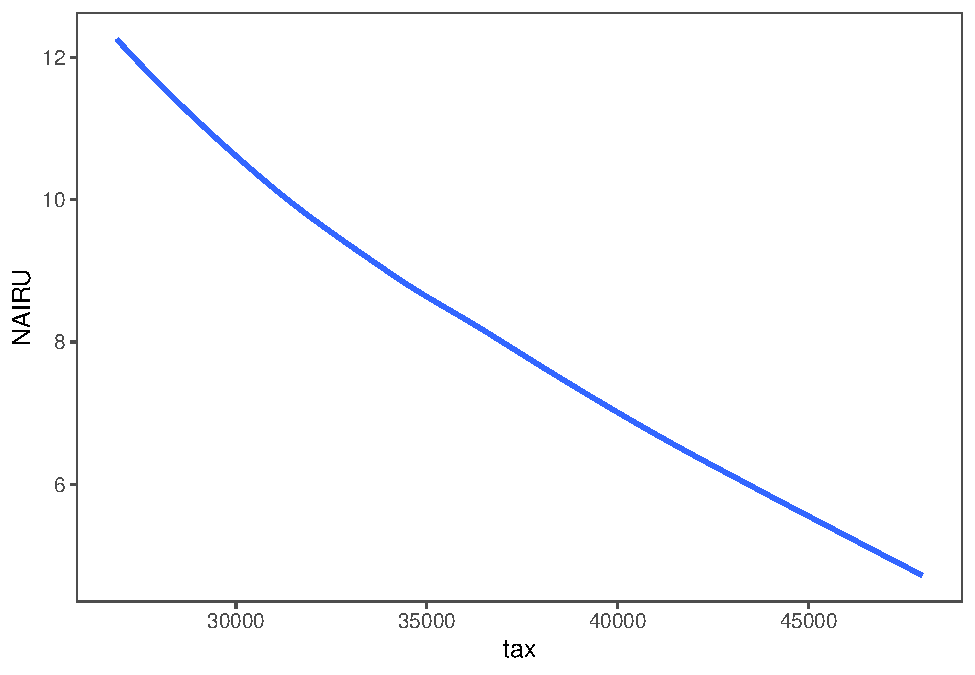
\includegraphics{Econo2_P5_files/figure-latex/loading data pme-2} \end{center}

\end{document}
